\chapter{Practice Retrieval}

Retrieval is a process of recalling what we have in memory. So, for our purposes, recall and retrieval refer to the same process. When we take tests or quizzes (or other such instruments), our minds attempt to recall answers (or relevant information that can be used to formulate an answer) to the questions we read.  Hopefully, we have previously stored this information in our brain (as a result of studying and learning) and can now recall it and write down the answer. To answer the questions then, we must recall the relevant information. Taking a test involves retrieval. Usually, our performance on a test is recorded and counts toward our final course grade.

\textbf{Practice Retrieval} refers to the fact that students should practice their retrieval skills prior to the test (or quiz or whatever). Wouldn't it be better to practice first, then take the real test?? Most people would answer yes. The figure below illustrates my concept of retrieval. Its really like getting information off of a diskette. [Putting information on the diskette (like saving a file) is called encoding when we refer to our memory. Encoding occurs during learning (hopefully).] Suggestions on how to perform practice retrieval are listed below the figure.

\begin{figure}
	\centering
	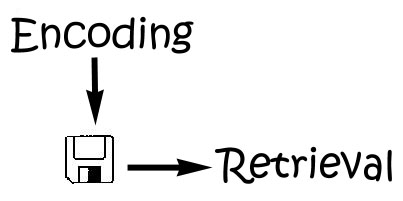
\includegraphics[width=0.55\linewidth]{./images/practice}
	\caption{Encoding and Retrieval}
	\label{fig:practice}
\end{figure}

\section{Suggestions}

\begin{itemize}
	\item Have a fellow student ask you questions as she reads her notes or looks in the textbook.
	\item Have a fellow student write down questions on a sheet of paper that you will answer later.
	\item Attempt to answer questions from old quizzes/tests.
	\item Visit Web sites of similar courses (to the one your in) and attempt to answer questions you find there.
\end{itemize}